\documentclass[bluish,slideColor,colorBG,pdf]{prosper}
\hypersetup{pdfpagemode=FullScreen}
\usepackage{graphicx}
\usepackage{epsfig}
\def\baselinestretch{1.0}
\setlength{\topmargin}{-60pt}
\setlength{\textheight}{460pt}
\setlength{\oddsidemargin}{0pt}
\setlength{\evensidemargin}{0pt}
\setlength{\textwidth}{660pt}
\setlength{\footskip}{0pt}
\parindent 0.3in
\hyphenpenalty=10000
\tolerance=10000
\pagestyle{empty}

\def\Prob{{\rm Prob\;}}
\def\prob{{\rm \;Prob\;}}


\author{January 2017}
\title{Genome 562}
\institution{Week 2}

\begin{document}

\maketitle

\begin{slide}[Replace]{A coalescent tree of copies of genes}

\centerline{\includegraphics[width=3.5in]{fig1-4.idraw}}

... such as you get if there is has been no recombination.
(We will discuss the theory of coalescents much later in the course).

\end{slide}

\begin{slide}[Replace]{If there is a mutation in locus A }

\centerline{\includegraphics[width=3.5in]{fig1-5.idraw}}

It exists in a clade on the tree.

\end{slide}

\begin{slide}[Replace]{ ... and one also in locus B }

\centerline{\includegraphics[width=3.5in]{fig1-6.idraw}}

It exists in another clade,

\end{slide}

\begin{slide}[Replace]{ ... or else where on the tree}

\centerline{\includegraphics[width=3.5in]{fig1-7.idraw}}

... or within the first clade,

\end{slide}

\begin{slide}[Replace]{ ... and even below the {\it A} clade}

\centerline{\includegraphics[width=3.5in]{fig1-8.idraw}}

... and can also have its clade include the clade for the first mutation.

\end{slide}

\begin{slide}[Replace]{So you get only three haplotypes}
\bigskip

The presence of three haplotypes is the sign that there need not have been any
recombination.  This is called the ``three-gamete test''.
\bigskip

\begin{itemize}
\item You can get both alleles at both loci from only two mutational events,
and ...
\item each creates one additional haplotype, so there is a total of 3
haplotypes, in which case
\item ... the $\mathsf{~D'~}$ measure of linkage disequilibrium is $\mathsf{~\pm
1~}$, 
\item ... so a perfect treelike genealogy goes along with LD as strong as
possible,
\item ... in other words, ``trees and $D$'s'' are telling you the same thing.
\end{itemize}

\end{slide}

\begin{slide}[Replace]{John Burdon Sanderson Haldane (1892 -- 1964) }

\begin{center}
\begin{tabular}{c c}
\includegraphics[height=1.2in]{haldane1930s.ps} &
\includegraphics[height=2in]{Haldane2.ps}\\
& \\
in the late 1930s & in the 1940s \\
\end{tabular}
\end{center}

\end{slide}

\begin{slide}[Replace]{JBS Haldane's achievements include ... }

\begin{itemize}
\item First to make tables of mixtures of gases for deep diving
\item First genetic mapping function (the Haldane Mapping Function, 1919)
\item Fundamental work in biochemical kinetics
\item In population genetics, basic equations for natural selection, migration, mutation
\item Pioneered use of likelihood methods in linkage estimation
\item One of first two to suggest (with Oparin) that the earth's early atmosphere was reducing
\item Early estimate of rate of mutation of a human gene
\item Advised British Admiralty on construction of World War II mini-subs
\item Science popularizations
\end{itemize}

\end{slide}

\begin{slide}[Replace]{Selection with haploids or multiplicative fitnesses}

\centerline{\psfig{figure=fig2-1.idraw,height=2.5in}}

\begin{center}
\parbox[t]{3.5in}{
Course of gene frequency change in haploid selection with initial
gene frequency $p_0  =  0.01$ and relative fitness 1.2 of the {\it A}
genotype.
}
\end{center}

\end{slide}

\begin{slide}[Replace]{Selection with dominance and recessiveness}

\centerline{\psfig{figure=fig2-2.idraw,height=2.3in}}

\begin{center}
\parbox[t]{3.5in}{
Change of the gene frequency plotted against gene frequency of {\it A} for
cases in which the favored allele is dominant (D), multiplicative (M) and
recessive (R).  Fitnesses of 
{\it AA} : {\it Aa} : {\it aa} genotypes were respectively 2.3 : 2.3 : 1,  5.29
: 2.3 : 1, and 2.3 : 1 : 1.
}
\end{center}

\end{slide}

\begin{slide}[Replace]{Change of gene frequency with or without dominance}

\centerline{\psfig{figure=fig2-3.idraw,height=2.5in}}

\begin{center}
\parbox[t]{3.5in}{
The course of gene frequency change over 50 generations when fitnesses of
{\it AA, Aa,} and {\it aa} are 2.3 : 2.3 : 1 (circles) and 2.3 : 1 : 1
(squares).  Initial frequency
of {\it A} is 0.02.
}
\end{center}

\end{slide}

\begin{slide}[Replace]{Change of gene frequency with overdominance}

\centerline{\psfig{figure=fig2-4.idraw,height=2.5in}}

\begin{center}
\parbox[t]{3.5in}{
The change in gene frequency ($\Delta p$) plotted against the gene
frequency in a case of overdominance where fitnesses of {\it AA : Aa : aa} are
0
.85 : 1 : 0.7.
}
\end{center}

\end{slide}

\begin{slide}[Replace]{Gene frequencies with overdominance}

\centerline{\psfig{figure=fig2-5.idraw,height=2.5in}}

\begin{center}
\parbox[t]{3.5in}{
Convergence of initial gene frequencies from $p_A  =  0.99$ and
$p_a  =  0.01$ to equilibrium when the fitnesses of {\it AA, Aa,} and
{\it aa} are $0.85 : 1 : 0.70$
}
\end{center}

\end{slide}

\begin{slide}[Replace]{Gene frequencies with underdominance}

\centerline{\psfig{figure=fig2-6.idraw,height=2.5in}}

\begin{center}
\parbox[t]{3.5in}{
Gene frequencies in successive generations when fitnesses of
$AA$, $Aa$, and $aa$ are underdominant (1.15 : 1 : 1.3) and the initial gene
frequency is 0.65(circles) or 0.68 (squares).
}
\end{center}

\end{slide}

\begin{slide}[Replace]{Mean fitness in a case of overdominance}

\centerline{\psfig{figure=fig2-8.ps,height=2.7in}}

\begin{center}
\parbox[t]{3.5in}{Mean fitness plotted as a function of gene frequency when fitnesses are: {\it AA} 0.55, {\it Aa} 1, {\it aa} 0.25.}
\end{center}

\end{slide}

\begin{slide}[Replace]{Mean fitness in a case of underdominance}

\centerline{\psfig{figure=fig2-6.5.idraw,height=2.7in}}

\begin{center}
\parbox[t]{3.5in}{Mean fitness plotted as a function of gene frequency when fitnesses are: {\it AA} 1.15, {\it Aa} 1, {\it aa} 1.30.}
\end{center}

\end{slide}

\begin{slide}[Replace]{Gene frequencies when fitnesses vary with time}

\centerline{\psfig{figure=fig2-9g.ps,height=2.2in}}

\begin{center}
\parbox[t]{3.5in}{Course of gene frequency change in a numerical example of acase of alternating Wet and Dry years (lighter lines) and in a case of random Wet and Dry years, independently drawn with equal probabilities. In both cases relative fitnesses of $A$ are 1.5 and 0.6 in Wet and Dry years.The starting gene frequency in both cases is 0.5.  }
\end{center}

\end{slide}

\end{document}
